%//==============================--@--==============================//%
\newpage
\subsection[3.4 Controlador PID]{\hspace*{0.075 em}\raisebox{0.2 em}{$\pmb{\drsh}$} Controlador PID}

\noindent ``Starting with simple proportional feedback, engineers early discovered integral control action as a means of eliminating bias offset. Then, finding poor dynamic response in many cases, an “anticipatory” term based on the derivative was added. The result is called the three-term or PID controller, and has the transfer function"\cite{FranklinPowell2015}

$$
    \boxed{D_c(s) = K_p + \dfrac{K_i}{s} + s \cdot K_d}
$$

\noindent Este controlador possui três ações ajustáveis --- Proporcional (\textbf{p}), Integral (\textbf{i}), Derivativa (\textbf{d}) --- com o objetivo de  melhorar a seguimento da referência e/ou rejeitar as perturbações e melhorar a resposta transitória.

%//==============================--@--==============================//%
\subsubsection[3.4.1 Ação proporcional]{$\pmb{\rightarrow}$ Ação proporcional}
\noindent Quando o sinal de controlo de realimentação é linearmente proporcional ao erro do sistema:
$$
    u(t) = K_p e(t)
$$

\noindent Designamos o resultado por retroação proporcional. Assim, o sinal de controlo varia linearmente com o erro do sistema. Se $K_p$ for grande o suficiente para obter um erro em regime estacionário adequadamente pequeno, \textbf{o amortecimento tornar-se-á demasiado pequeno} para a obtenção de uma resposta transitória satisfatória (apenas com controlo proporcional)

\begin{figure}[H]
    \centering
    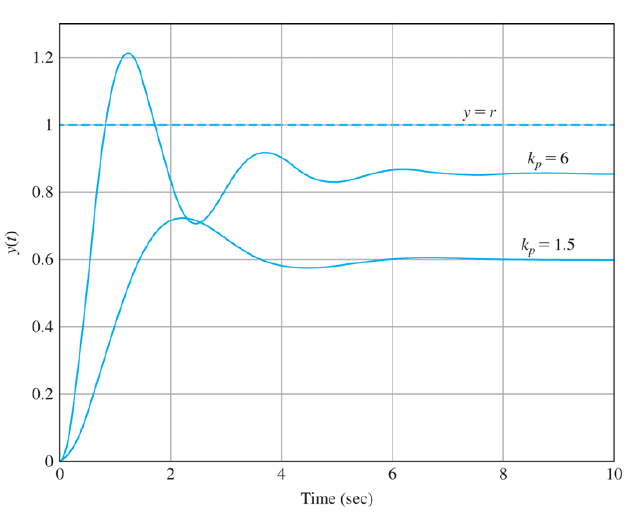
\includegraphics[width = 0.5\linewidth]{img/3/proportional-control.png}
    \caption{Efeito da ação proporcional para vários valores de $K_p$.}
    \label{fig:proportional-control}
\end{figure}

%//==============================--@--==============================//%
\subsubsection[3.4.2 Ação integral]{$\pmb{\rightarrow}$ Ação integral}
\noindent Quando um sinal de controlo de realimentação é linearmente proporcional ao integral do erro do sistema, chamamos ao resultado \textbf{realimentação integral}. 
$$
    u(t) = K_i \int e(\tau)\, d\tau
$$

\noindent $K_i$ designa-se ganho integral. A ação integral garante que, o sinal de controlo, em cada instante de tempo é um somatório de todos os valores passados do erro de seguimento.

\begin{figure}[H]
    \centering
    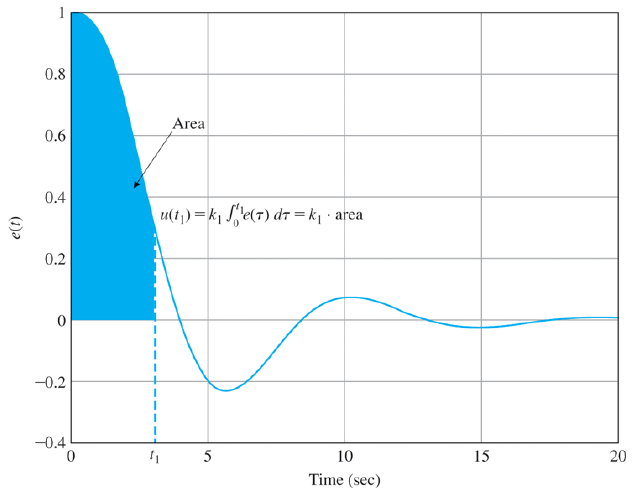
\includegraphics[width = 0.5\linewidth]{img/3/integral-control.png}
    \caption{``Integral control is based on the history of the system error"\cite{FranklinPowell2015}.}
    \label{fig:integral-control}
\end{figure}

\noindent A ação integral tem a principal virtude de poder fornecer um valor finito de controlo com erro de seguimento nulo. Tal acontece porque $u(t)$ é uma função de todos os valores passados de $e(t)$ e não apenas do valor no instante atual. Admitindo que o sistema da \hyperref[fig:feed-loop]{fig.6} possui um controlador integral, obtemos:

$$
    \dfrac{E(s)}{R(s)} = \dfrac{s}{s + K_i G(s)}\qquad
    \dfrac{Y(s)}{R(s)} = \dfrac{K_i G(s)}{s + K_i G(s)}\qquad
    \dfrac{U(s)}{R(s)} = \dfrac{K_i}{s + K_i G(s)}
$$

\noindent Assumindo como entrada o degrau unitário e aplicando o teorema do valor final:

$$
    e(\infty) = 0\quad
    y(\infty) = 1\quad
    u(\infty) = 1
$$
\noindent Note-se que o erro de seguimento em regime estacionário será zero, qualquer que seja o valor de $K_i$. O ganho integral $K_i$ é meramente selecionado para proporcionar uma resposta dinâmica aceitável. aceitável; no entanto, O seu incremento excessivo poderá causar instabilidade. Neste sentido podemos afirmar o seguinte:

\begin{itemize}
    \item melhor seguimento em regime permanente.
    \item pior estabilidade relativa --- os pólos infletem para o s.p.c.d com o aumento de $K_i$.
\end{itemize}

\noindent Consequentemente é relevante falar do \textbf{controlador integral proporcional}:
$$
    K_p \cdot \left[1 + \dfrac{1}{T_s s}\right] = K_p \cdot \dfrac{s + 1/T_s}{s}
$$

\begin{itemize}
    \item melhor seguimento em regime permanente.
    \item zero em $s = -1/T_s$, normalmente colocado perto do pólo referente ao integrador de modo a não destabilizar a dinâmica do sistema.
    \item \textbf{melhora o seguimento em regime permanente}, sem alterar significativamente os ramos principais do root-locus.
\end{itemize}
%//==============================--@--==============================//%
\newpage
\subsubsection[3.4.3 Ação derivativa]{$\pmb{\rightarrow}$ Ação derivativa}
\noindent O objetivo da ação derivativa é melhorar a estabilidade do sistema em malha fechada, bem como acelerar a resposta transitória e reduzir o \textit{overshoot}.

$$
    u(t) = K_d \Dot{e}(t)
$$

\noindent A ação derivativa quase nunca é utilizado por si só, é assim relevante referir o \textbf{controlador porporcional derivativo} e o \textbf{controlador proporcional integral derivativo}, respetivamente:

\vspace{1em}
\noindent \textbf{Controlador porporcional derivativo}
$$
    K_pT_d\cdot(s + 1/T_d)
$$
\begin{itemize}
    \item “atrai” os ramos do root-locus afastando-os do s.p.c.d --- aumenta $\gamma$ (amortecimento)
    \item introduz “antecipação” --- $u(t)$ depende não só da intensidade do erro $e(t)$ (\textbf{ação P}), mas também da sua rapidez de variação (\textbf{ação D}).
    \item amplifica as componentes de alta frequência dos sinais.
\end{itemize}

\noindent \textbf{Controlador proporcional integral derivativo}
$$
    K_pT_d\cdot(s + 1/T_d)\cdot \dfrac{(s + 1/T_i)}{s}
$$
\begin{itemize}
    \item Reúne as ações anteriores.
    \item Partindo do controlador PD, introduz-se um polo na origem e um zero perto da origem.
    \item A substituição PD por PID melhora o seguimento em regime permanente, sem alterar significativamente os ramos principais do root-locus.
\end{itemize}

{
\mdfsetup{linewidth=2pt}

\begin{mdframed}
    \noindent O desenho de um controlador envolve sempre a implementação inicial de um controlador Proporcional-Derivativo (\textbf{PD}), que é responsável pelas características transitórias do sistema. Tal é seguido pela implementação de um controlador Proporcional-Integral (\textbf{PI}) para eliminar o erro em regime estacionário.
\end{mdframed}
}